\section{Results}\label{sec:results}
% Show the result/capabilities of your solution through plots, tables, screenshots, videos, etc.
\begin{figure}[H]
\centering
\begin{subfigure}[b]{0.3\textwidth}
    \centering
    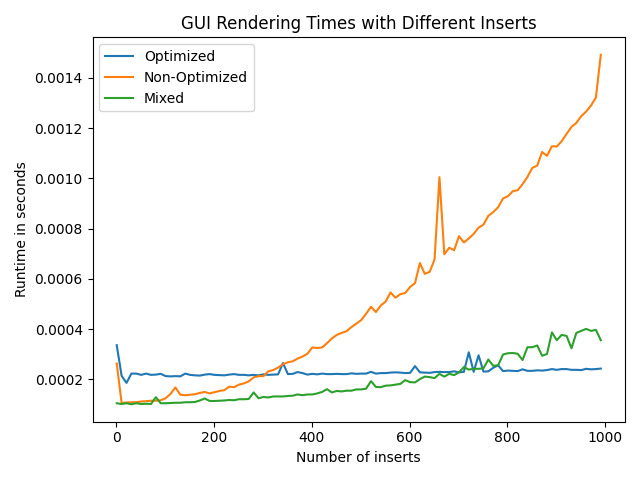
\includegraphics[width=\textwidth]{./images/Profiler-Render-Metric-Size1.jpg}
    \label{fig:renderMetric}
\end{subfigure}
\hfill
\begin{subfigure}[b]{0.3\textwidth}
    \centering
    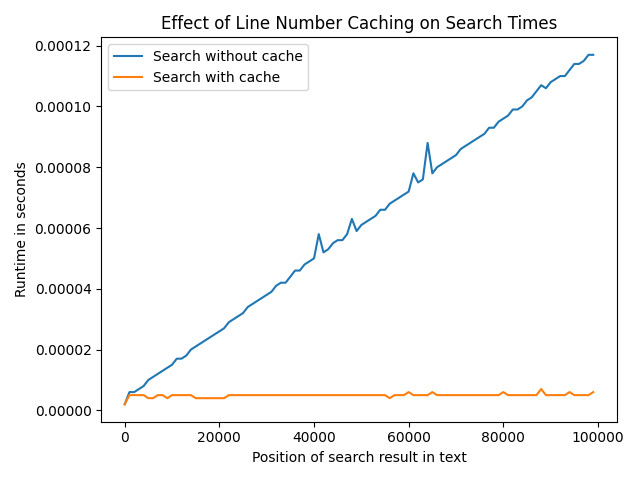
\includegraphics[width=\textwidth]{./images/Profiler-Find-Caching.jpg}
    \label{fig:findMetric}
\end{subfigure}
\hfill
\begin{subfigure}[b]{0.3\textwidth}
    \centering
    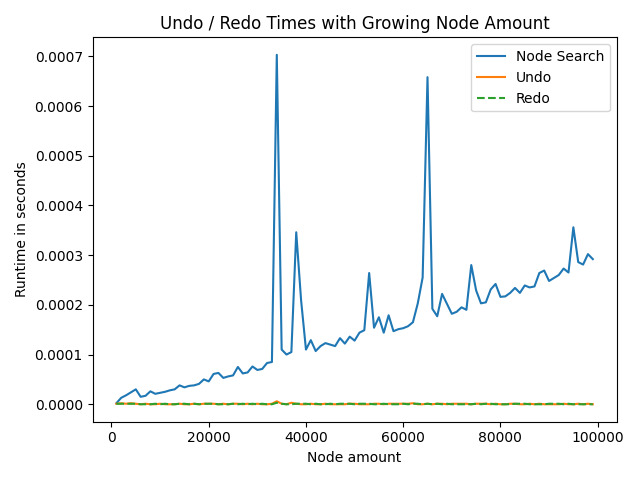
\includegraphics[width=\textwidth]{./images/Profiler-Undo-Redo.jpg}
    \label{fig:undoMetric}
\end{subfigure}
\label{fig:codeStructure}
\end{figure}

%GUI
\begin{figure}[h]
    \centering
    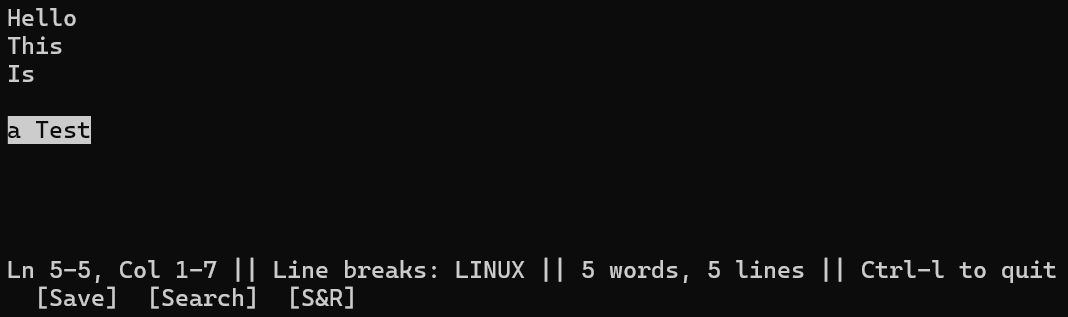
\includegraphics[width=1.0\linewidth]{figures/results_terminal.png}
    \caption{GUI of our text editor running on WSL}
    \label{fig:GUIterminal}            
\end{figure}
\noindent
Above you can see our GUI. From the top left you can see 5 lines written, one of the blank.
\\'a Test' is marked and can be use to copy/paste or delete this section.
Ln 5-5 means marked are rows from 5 to 5, same for Col but column 1 to 7.
'Line breaks: LINUX' means that the current line break style used is LINUX ($\backslash$n). It also supports MSDOS ($\backslash$r$\backslash$n) and MAC ($\backslash$r).
\\Next to it you also have total line and total word count and to the right is the short-cut to exit the editor.
At the very bottom are buttons that you can press to use them. S\&R means search and replace.
\\All aspetcs of our GUI will be shown in this video \cite{demo}, as some of these things are impractical to show on a picture.